\documentclass[11pt]{article}

\usepackage[margin=1in]{geometry}
\usepackage{graphicx}
\usepackage{booktabs}
\usepackage{amsmath,amssymb}
\usepackage{multirow}
\usepackage{hyperref}
\usepackage{float}
\usepackage{caption}
\usepackage{subcaption}
\usepackage{enumitem}
\usepackage{setspace}
\usepackage{tikz}
\usetikzlibrary{positioning,arrows.meta,shapes.geometric}

\graphicspath{{../Solution/}{../Solution/open_set_outputs/}}

\setstretch{1.0}

\begin{document}

\begin{titlepage}
\clearpage\thispagestyle{empty}
\centering
\vspace{1cm}

\rule{\linewidth}{1mm} \\[0.5cm]
{ \Large \bfseries ISyE 6740 -- Summer 2026\\[0.2cm]
Final Report}\\[0.5cm]
\rule{\linewidth}{1mm} \\[1cm]

\begin{tabular}{l p{9cm}}
\textbf{Team Member Names:} & Aswath Oruganti, Bakiye Hilal Khaniyev, Yussif Salama \\[10pt]
\textbf{Group:} & 016 \\[10pt]
\textbf{Project Title:} & Open-Set Recognition of Plant Species: Detecting Unfamiliar Flora for Biodiversity Screening \\[10pt]
\end{tabular}

\vfill
\end{titlepage}

\begin{abstract}
\noindent
Automated plant identification systems are almost universally closed-set: they assign every image to one of the species seen during training, and cannot report that a specimen is unfamiliar. For biodiversity screening this is precisely backwards, since the observations that most warrant expert attention are the ones absent from the training data. We study open-set recognition on Pl@ntNet-300K, curating the dataset to 226 well-represented species, training on 181 of them, and withholding 45 entirely so that ground truth for novelty detection is exact by construction. Using ResNet-18 and EfficientNet-B0 as feature extractors, we compare seven methods for scoring how unfamiliar an image is. Distance-based scorers on length-normalized embeddings clearly win: $k$-nearest neighbour distance reaches 0.790 ROC AUC against 0.620 for the standard maximum-softmax-probability baseline, with non-overlapping species-level bootstrap intervals. Length normalization alone is worth up to 12 AUC points, exceeding the benefit of the larger backbone. Our most instructive result is negative: One-Class SVM and Isolation Forest perform at or below chance. Two controlled ablations locate the cause. Removing embedding magnitude does not rescue them, refuting the intuitive explanation, whereas replacing 181 class centroids with a single global centroid -- holding metric and preprocessing fixed -- reproduces the failure almost exactly, moving AUC by 0.40. Unfamiliar species do not lie outside the region occupied by the training data; they lie in the gaps between known class clusters, which are invisible to any method that models that region as a whole. Finally, detection difficulty depends strongly on taxonomy: AUC falls from 0.897 for species from an unseen genus to 0.748 for species whose genus the model already knows, so the hard case is recognizing a new species among its own known relatives. At a false positive rate of 0.69 for 95\% recall, such a system is best deployed to rank observations for expert triage rather than to filter them automatically.
\end{abstract}

\section*{Team Member Contributions}

\begin{itemize}[leftmargin=1.2cm]
    \item \textbf{Aswath Oruganti:} Built the data curation pipeline that filters Pl@ntNet-300K down to well-represented species and forms the disjoint known/unknown species split. Implemented and fine-tuned both classification backbones, ResNet-18 and EfficientNet-B0, and produced the representation-analysis visualizations for each (mutual information, PCA projections, and activation fingerprints).
    
    \item \textbf{Bakiye Hilal Khaniyev:} Designed the open-set evaluation protocol, including the balanced 2,000-versus-2,000 test set and the restriction to held-out images, so that no training image can inflate the known-class scores. Implemented the shared embedding extraction and export pipeline used by both backbones, interpreted the representation analysis, and wrote the final report.
    
    \item \textbf{Yussif Salama:} Implemented and evaluated all seven open-set scorers, from the softmax and energy baselines to the distance-based and one-class methods, and diagnosed the one-class failure through the normalization and class-conditioning ablations. Added the extended evaluation: detailed closed-set metrics, the taxonomic-distance analysis, species-level bootstrap intervals, and the openness sweep.
\end{itemize}

\newpage

\section{Problem Statement}


Accurate identification of plant species from photographs has become increasingly important for biodiversity monitoring, ecological research, conservation efforts, and citizen science applications. Recent advances in deep learning, particularly convolutional neural networks (CNNs), have substantially improved automated plant classification, with several publicly available models now achieving high accuracy on large-scale image datasets. These systems are increasingly being integrated into mobile applications and biodiversity platforms to assist both researchers and the general public in species identification.

Despite these advances, most existing image classification systems operate under the closed-set assumption: every test image is assumed to belong to one of the species observed during training. In practice, however, this assumption rarely holds. Natural ecosystems contain many species that are absent from the training data, whether because they are rare, newly introduced, geographically localized, or simply underrepresented in existing datasets. Conventional classifiers are nevertheless forced to assign these unfamiliar observations to one of the known classes, often producing highly confident but incorrect predictions.

This limitation presents a significant challenge for biodiversity screening. In many ecological applications, recognizing that a specimen is unfamiliar can be more valuable than assigning an incorrect species label. Flagging observations that fall outside the model's learned knowledge allows experts to prioritize potentially novel or unusual specimens for further investigation instead of spending effort correcting erroneous predictions.

This project investigates the problem of open-set recognition for plant species identification. Rather than attempting to classify every possible plant species, we train image classification models on a curated subset of well-represented species and evaluate their ability to distinguish between known and previously unseen species. The study combines deep feature extraction using modern convolutional neural networks with several open-set recognition techniques operating in the learned embedding space.

Specifically, we compare feature representations learned by ResNet-18 and EfficientNet-B0 and evaluate seven strategies for detecting unfamiliar species: Maximum Softmax Probability, the energy score, Mahalanobis distance with and without length normalization, $k$-nearest neighbour distance, One-Class Support Vector Machines, and Isolation Forest. The objective is not only to obtain high classification accuracy on known species but also to determine which open-set recognition methods most effectively identify species that were intentionally excluded from the training process. Such a system could provide a practical first-pass screening tool for biodiversity monitoring by automatically identifying observations that warrant expert review.

Our results show that the choice of detection method matters more than the choice of architecture, that normalizing embeddings to unit length is the single most valuable preprocessing step, and that the widely used one-class anomaly detectors fail on this task for a reason we are able to diagnose directly from the geometry of the embedding space.

\section{Related Work}

Deep convolutional neural networks have become the dominant approach for image-based plant species identification, largely due to the availability of large annotated datasets and advances in transfer learning. The Pl@ntNet-300K dataset introduced by Garcin et al.~\cite{garcin2021plantnet} is one of the largest publicly available plant image datasets and has become a standard benchmark for evaluating plant classification algorithms. However, the dataset exhibits a highly long-tailed class distribution, making accurate recognition of infrequently observed species particularly challenging.

Transfer learning has significantly improved image classification performance by allowing models pretrained on ImageNet to learn domain-specific representations using relatively limited task-specific data. Residual Networks (ResNet)~\cite{he2016deep} introduced skip connections that enable the successful training of deep neural networks, while EfficientNet~\cite{tan2019efficientnet} demonstrated that carefully balancing network depth, width, and input resolution can substantially improve both predictive accuracy and computational efficiency. Both architectures have been successfully applied across numerous fine-grained image classification tasks, including biodiversity monitoring.

While these models achieve strong performance under the closed-set assumption, they remain unable to recognize observations belonging to previously unseen classes. Open-set recognition addresses this limitation by enabling models to identify inputs that fall outside the training distribution. Hendrycks and Gimpel~\cite{hendrycks2017baseline} proposed Maximum Softmax Probability (MSP) as a simple baseline for out-of-distribution detection using classification confidence. Because softmax normalization discards the absolute scale of the logits, Liu et al.~\cite{liu2020energy} instead derived an energy score from the full logit vector, which corresponds to an unnormalized log-density under the classifier and is consistently better calibrated for novelty.

A second line of work exploits the geometry of the learned feature space rather than the classifier output. Lee et al.~\cite{lee2018simple} model each class as a Gaussian and score inputs by Mahalanobis distance to the nearest class, which requires estimating a covariance matrix that is singular in high-dimensional embedding spaces and therefore depends on shrinkage estimators such as that of Ledoit and Wolf~\cite{ledoit2004well}. Sun et al.~\cite{sun2022knnood} showed that a fully non-parametric alternative, the distance to the $k$ nearest training embeddings under a normalized feature space, matches or exceeds these parametric methods while making no assumption about class shape. A third family dispenses with class labels entirely and treats novelty as anomaly detection over the pooled training features, using One-Class Support Vector Machines~\cite{scholkopf2001estimating} to estimate the support of the known distribution or Isolation Forests~\cite{liu2008isolation} to identify points in sparse regions.

These method families are usually benchmarked on coarse out-of-distribution tasks, where the novel inputs come from a visibly different dataset. Fine-grained open-set recognition, in which the novel classes are drawn from the same domain and often the same genus as the known ones, is a substantially harder regime and one where the relative standing of these methods is less well established.

Building on this prior work, our study combines deep feature representations learned through transfer learning with multiple open-set recognition techniques to evaluate their effectiveness for biodiversity screening. Rather than focusing solely on closed-set classification accuracy, we emphasize the ability to reliably identify plant species that were intentionally excluded from the training process, and we additionally characterize \emph{when} these methods fail: which geometric property of the embedding space causes the one-class detectors to break down, and how detection difficulty scales with taxonomic distance between the novel species and the training set.


\section{Data Source and Preparation}

\subsection{PlantNet-300K Dataset}

This study used the Pl@ntNet-300K dataset~\cite{garcin2021plantnet}, a large-scale public benchmark for plant image classification containing 306,146 images spanning 1,081 plant species. The images were collected through the Pl@ntNet citizen science platform and exhibit substantial variability in viewpoint, lighting conditions, background clutter, image quality, and developmental stage of the plants. Consequently, the dataset closely reflects the challenges encountered in real-world biodiversity monitoring.

One characteristic of Pl@ntNet-300K is its highly long-tailed class distribution. While a relatively small number of species are represented by thousands of images, many species contain only a handful of observations. Such imbalance makes supervised training difficult and can bias classification models toward the most frequently occurring species.

\subsection{Dataset Curation}

To obtain a sufficiently large and well-supported training set, we curated the dataset by selecting only the most image-rich species. Approximately the top 20\% of species ranked by image count were retained, while species with very few observations were excluded from the supervised training process. This curation reduced the impact of severe class imbalance and ensured that each retained class contained enough samples for effective transfer learning.

Following curation, the retained species were randomly partitioned at the \emph{species level} into two disjoint groups: \textit{known} species and \textit{unknown} species. Images belonging to the unknown species were completely removed from model training and validation. Consequently, the model never observed these species during learning, allowing them to serve as genuine unseen classes during evaluation.

For the known species, the dataset's predefined training, validation, and test splits were preserved. The training set was used for fine-tuning the convolutional neural networks, the validation set was used for model selection and hyperparameter tuning, and the held-out test set was reserved exclusively for the final evaluation.

The open-set evaluation dataset consisted of two components:
\begin{enumerate}
    \item test images belonging to the known species, which should be correctly classified by the model, and
    \item images belonging to the held-out unknown species, which should be identified as unfamiliar rather than assigned to a known class.
\end{enumerate}

Constructing the evaluation dataset in this manner provides exact ground truth for both closed-set classification and open-set detection, while preventing information leakage between the training and testing stages.

\begin{figure}[H]
\centering
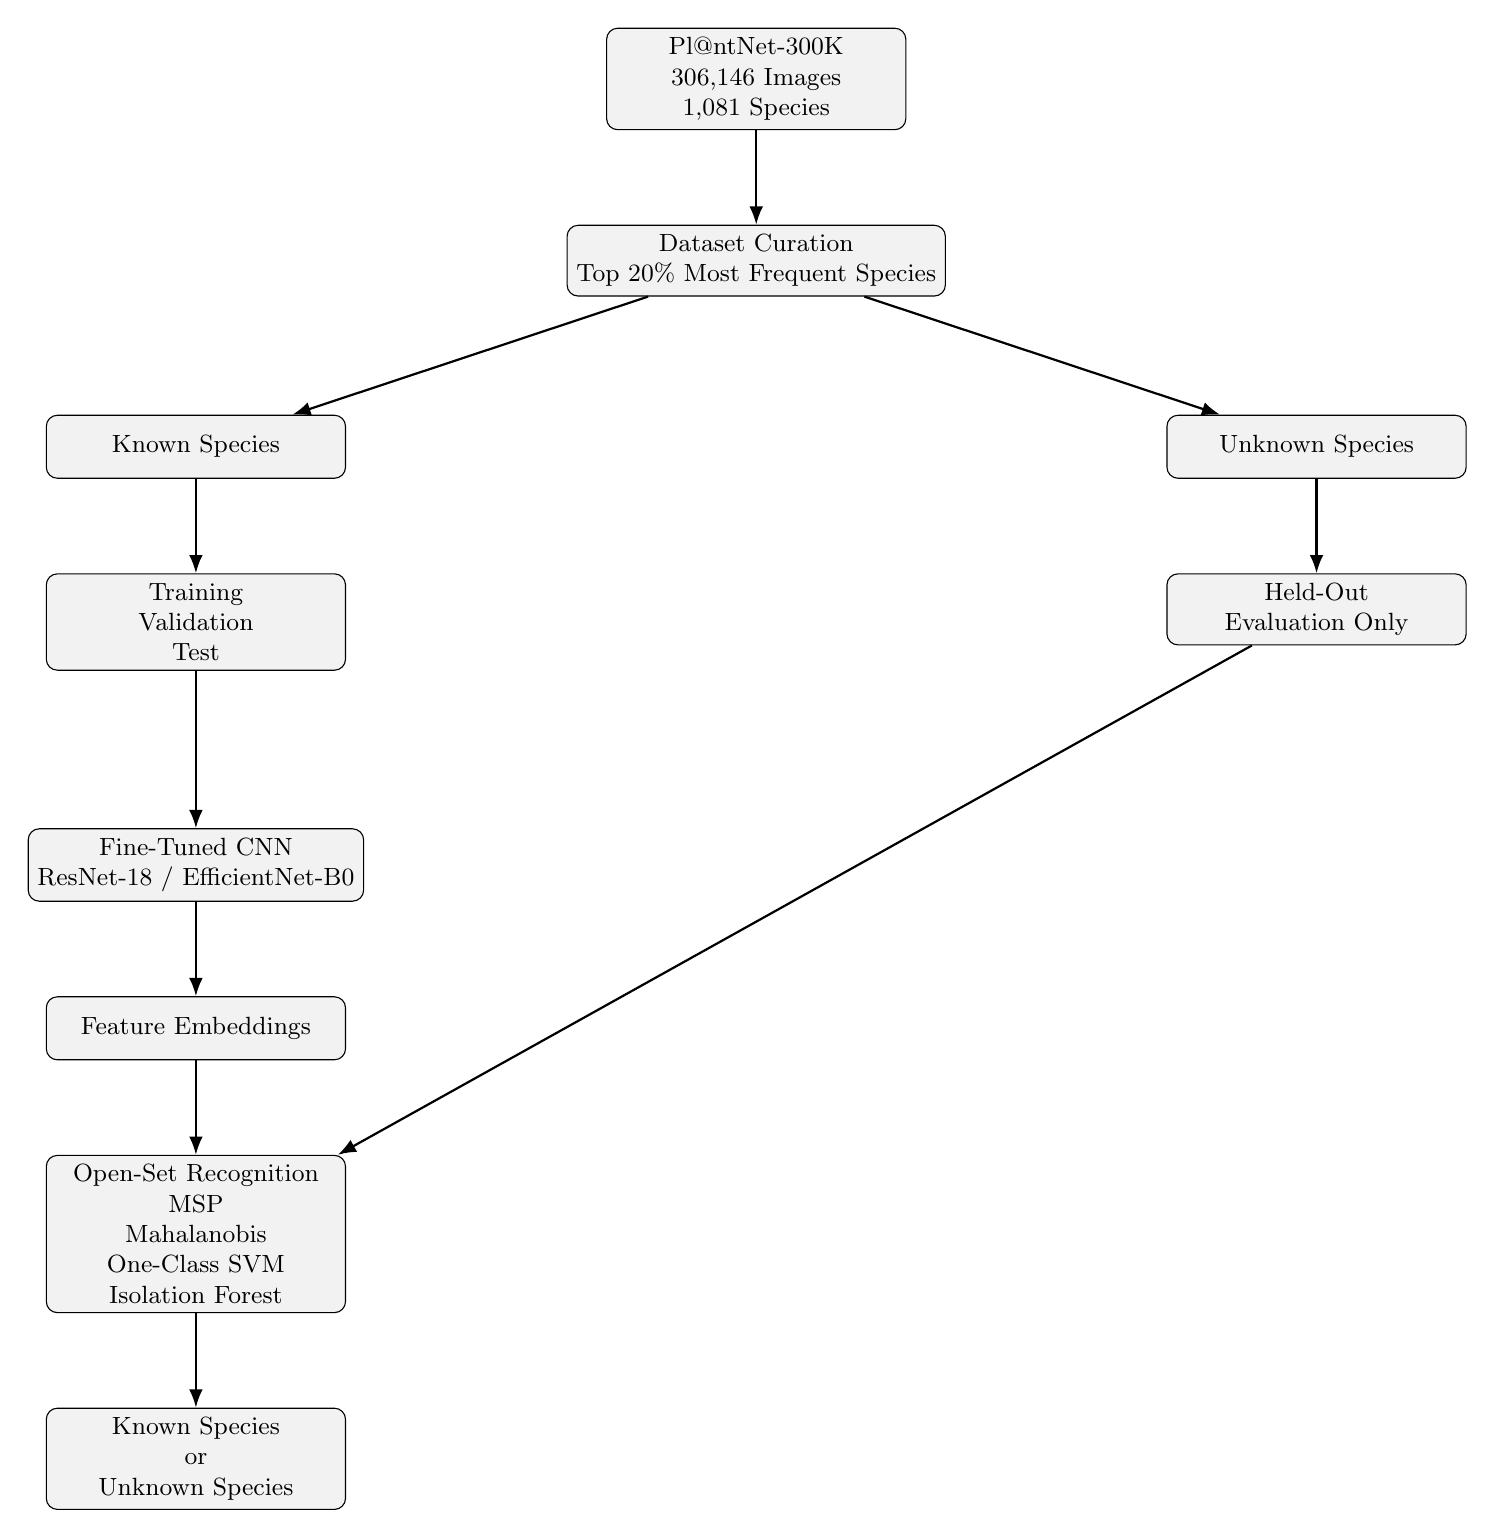
\begin{tikzpicture}[
node distance=1.2cm,
>=Latex,
every node/.style={font=\small},
box/.style={
draw,
rounded corners,
align=center,
minimum width=3.8cm,
minimum height=0.8cm,
fill=gray!10
},
arrow/.style={->,thick}
]

% Main dataset
\node[box] (dataset) {Pl@ntNet-300K\\306,146 Images\\1,081 Species};

% Curation
\node[box, below=of dataset] (curated)
{Dataset Curation\\Top 20\% Most Frequent Species};

% Split
\node[box, below left=1.5cm and 2.8cm of curated] (known)
{Known Species};

\node[box, below right=1.5cm and 2.8cm of curated] (unknown)
{Unknown Species};

% Known split
\node[box, below=of known] (train)
{Training\\Validation\\Test};

% Unknown test
\node[box, below=of unknown] (unktest)
{Held-Out\\Evaluation Only};

% CNN
\node[box, below=2cm of train] (cnn)
{Fine-Tuned CNN\\ResNet-18 / EfficientNet-B0};

% Embeddings
\node[box, below=of cnn] (embed)
{Feature Embeddings};

% Open-set
\node[box, below=of embed] (osr)
{Open-Set Recognition\\MSP\\Mahalanobis\\One-Class SVM\\Isolation Forest};

% Output
\node[box, below=of osr] (output)
{Known Species\\or\\Unknown Species};

% Arrows
\draw[arrow] (dataset)--(curated);

\draw[arrow] (curated)--(known);
\draw[arrow] (curated)--(unknown);

\draw[arrow] (known)--(train);
\draw[arrow] (train)--(cnn);
\draw[arrow] (cnn)--(embed);
\draw[arrow] (embed)--(osr);
\draw[arrow] (osr)--(output);

\draw[arrow] (unktest)--(osr);
\draw[arrow] (unknown)--(unktest);

\end{tikzpicture}

\caption{Overview of the proposed open-set recognition framework. The PlantNet-300K dataset is first curated to retain the most well-represented species. The retained species are divided into known and unknown groups. Only known species are used for model training, while unknown species are reserved exclusively for evaluation. Feature embeddings extracted from the fine-tuned CNN are used by several open-set recognition methods to determine whether an input belongs to a known species or should be flagged as unfamiliar.}
\label{fig:pipeline}
\end{figure}


\section{Methodology}

Our proposed framework combines supervised image classification with open-set recognition to identify plant species that were not observed during training. The overall workflow is illustrated in Figure~\ref{fig:pipeline}. A convolutional neural network is first fine-tuned to classify the known plant species while simultaneously learning discriminative feature representations. These learned embeddings are then used by several open-set recognition algorithms to determine whether a test image belongs to one of the known species or should instead be classified as unfamiliar.

\subsection{Feature Learning}

Two convolutional neural network architectures were investigated in this study: ResNet-18~\cite{he2016deep} and EfficientNet-B0~\cite{tan2019efficientnet}. Both models were initialized with ImageNet-pretrained weights and fine-tuned on the curated set of known plant species using transfer learning.

Beyond their role as classifiers, both networks served as feature extractors. After training, feature vectors were obtained from the penultimate layer for every image. These embeddings provide a compact representation of visual characteristics and form the basis for all subsequent open-set recognition methods.

\subsection{Open-Set Evaluation Protocol}

Species assigned to the unknown set were completely excluded from training and validation. During evaluation, the test dataset consisted of two groups:

\begin{enumerate}
    \item Images belonging to known species, which should be correctly classified.
    \item Images belonging to unknown species, which should be identified as unfamiliar.
\end{enumerate}

This evaluation protocol ensures that unknown species remain entirely unseen during model training, thereby preventing information leakage and providing an unbiased assessment of open-set recognition performance.

\subsection{Problem Formulation}
\label{sec:formulation}

We state the task formally before describing the individual methods. Let $\mathcal{Y}_{\text{known}} = \{1, \dots, C\}$ denote the $C = 181$ species used for training and $\mathcal{Y}_{\text{unknown}}$ the disjoint set of 45 withheld species, so that $\mathcal{Y}_{\text{known}} \cap \mathcal{Y}_{\text{unknown}} = \emptyset$. The fine-tuned network provides two mappings: an embedding function $f: \mathcal{X} \to \mathbb{R}^d$ taking an image to its penultimate-layer representation, with $d = 512$ for ResNet-18 and $d = 1280$ for EfficientNet-B0, and a linear head producing logits
\begin{equation}
z(x) = W f(x) + b, \qquad W \in \mathbb{R}^{C \times d}, \quad b \in \mathbb{R}^{C}.
\end{equation}

A conventional closed-set classifier returns $\hat{y}(x) = \arg\max_j z_j(x)$ and is structurally incapable of expressing that $x$ belongs to no class in $\mathcal{Y}_{\text{known}}$. Open-set recognition augments it with a scalar \emph{unfamiliarity score} $s: \mathcal{X} \to \mathbb{R}$ and a threshold $\tau$, giving the decision rule
\begin{equation}
\hat{y}_{\text{open}}(x) =
\begin{cases}
\text{``unfamiliar''} & \text{if } s(x) > \tau, \\[2pt]
\arg\max_j z_j(x) & \text{otherwise.}
\end{cases}
\end{equation}

Every method below is one choice of $s$, and all are oriented so that larger values indicate greater novelty. The central empirical question is which choice of $s$ best separates images of $\mathcal{Y}_{\text{known}}$ from images of $\mathcal{Y}_{\text{unknown}}$. Because ROC AUC is invariant to any strictly increasing transformation of $s$, the comparison is independent of $\tau$ and of the arbitrary scale of each score.

Two further quantities recur below. Writing $\mathcal{D}_c = \{f(x_i) : y_i = c\}$ for the training embeddings of class $c$, we use the class means $\mu_c = |\mathcal{D}_c|^{-1} \sum_{v \in \mathcal{D}_c} v$ and the projection onto the unit sphere
\begin{equation}
\tilde{f}(x) = \frac{f(x)}{\lVert f(x) \rVert_2},
\label{eq:l2norm}
\end{equation}
which discards the magnitude of the embedding and retains only its direction. The role of Equation~\eqref{eq:l2norm} turns out to be central to our results.

\subsection{Open-Set Recognition Methods}

To distinguish familiar and unfamiliar species, several complementary open-set recognition methods were investigated. They fall into three families. The first operates on the classifier's output logits (MSP and Energy), the second models the geometry of the known classes in the embedding space (Mahalanobis and $k$-nearest neighbours), and the third treats the entire set of known embeddings as a single distribution whose support must be estimated (One-Class SVM and Isolation Forest). Only the second family uses the class labels of the known species.

\subsubsection{Maximum Softmax Probability}

Maximum Softmax Probability (MSP)~\cite{hendrycks2017baseline} serves as a simple baseline, interpreting the classifier's largest softmax output as its confidence:
\begin{equation}
s_{\text{MSP}}(x) = 1 - \max_{j} \frac{\exp\!\big(z_j(x)\big)}{\sum_{l=1}^{C} \exp\!\big(z_l(x)\big)}.
\end{equation}
Its known weakness is that the softmax normalization discards the overall magnitude of the logits, retaining only their relative sizes, so a confidently wrong prediction on an unfamiliar input is indistinguishable from a confidently correct one.

\subsubsection{Energy Score}

The energy score~\cite{liu2020energy} instead summarizes the entire logit vector,
\begin{equation}
s_{\text{energy}}(x) = -\log \sum_{j=1}^{C} \exp\!\big(z_j(x)\big),
\end{equation}
which is the negative log-partition function of the classifier's implied Gibbs distribution and is therefore proportional to the unnormalized log-density of $x$ under the model. Because it preserves the absolute scale of the logits that MSP normalizes away, it is less affected by the overconfidence that softmax probabilities exhibit.

\subsubsection{Mahalanobis Distance}

Mahalanobis distance~\cite{lee2018simple} models each known class as a Gaussian in embedding space and scores an image by its distance to the nearest such class:
\begin{equation}
s_{\text{maha}}(x) = \min_{c \in \mathcal{Y}_{\text{known}}} \sqrt{\big(f(x) - \mu_c\big)^{\!\top} \Sigma^{-1} \big(f(x) - \mu_c\big)}.
\end{equation}
A single covariance $\Sigma$ is shared across all classes and estimated from the pooled within-class residuals $\{f(x_i) - \mu_{y_i}\}$. Per-class covariances are unusable here: with $d = 512$ or $1280$ dimensions but only about 270 training images per class, each per-class scatter matrix is singular and cannot be inverted. We therefore estimate $\Sigma$ with the Ledoit--Wolf shrinkage estimator~\cite{ledoit2004well}, which shrinks the sample covariance toward a scaled identity by an analytically optimal amount and guarantees a well-conditioned, invertible result.

This scorer was evaluated both on the raw embeddings $f(x)$ and on the normalized embeddings $\tilde{f}(x)$ of Equation~\eqref{eq:l2norm}.

\subsubsection{$k$-Nearest Neighbour Distance}

The $k$-nearest neighbour scorer~\cite{sun2022knnood} is non-parametric, making no assumption about the shape of each class. Letting $\mathrm{NN}_k(x)$ denote the $k$ training embeddings closest to $x$,
\begin{equation}
s_{k\text{NN}}(x) = \frac{1}{k} \sum_{v \in \mathrm{NN}_k(x)} \big\lVert \tilde{f}(x) - v \big\rVert_2,
\end{equation}
with $k = 5$ and normalized embeddings throughout. Because it measures \emph{local} density rather than distance to a class centroid, it can represent classes whose images form several distinct clusters, which is common for a plant species photographed as flower, leaf, fruit, and whole plant.

\subsubsection{One-Class Support Vector Machine}

One-Class SVM~\cite{scholkopf2001estimating} estimates the support of the known-embedding distribution directly, solving
\begin{equation}
\min_{w, \rho, \xi} \; \tfrac{1}{2}\lVert w \rVert^2 + \frac{1}{\nu n}\sum_{i=1}^{n} \xi_i - \rho
\quad \text{s.t.} \quad \langle w, \phi(v_i) \rangle \geq \rho - \xi_i, \;\; \xi_i \geq 0,
\end{equation}
where $\phi$ is the feature map of an RBF kernel and $\nu = 0.1$ bounds the fraction of training points allowed to fall outside the estimated support. The unfamiliarity score is the negated decision function, $s_{\text{OCSVM}}(x) = \rho - \langle w, \phi(f(x)) \rangle$, so points outside the support score highest.

\subsubsection{Isolation Forest}

Isolation Forest~\cite{liu2008isolation} takes an entirely different route, recursively partitioning the space with 200 randomized axis-aligned splits and measuring how quickly each point becomes isolated. Points requiring few splits lie in sparse regions and are scored as anomalous, with $s_{\text{IF}}(x)$ the negated normalized path length averaged over the ensemble.

Both one-class methods were fitted on standardized embeddings, since neither is scale-invariant. Crucially, both estimate a \emph{single global} region of normality and make no use of the class labels, in contrast to Mahalanobis distance and $k$-nearest neighbours, which model the $C$ known classes separately. Section~\ref{sec:discussion} shows that this distinction is what determines whether a method succeeds.

\subsection{Evaluation Metrics}

Open-set detection was treated as a binary decision problem in which the positive class is ``unfamiliar''. Because every method produces a continuous score, performance was measured primarily with threshold-free metrics, avoiding any dependence on an arbitrarily chosen operating point.

The area under the receiver operating characteristic curve (ROC AUC) measures the probability that a randomly chosen unknown-species image receives a higher unfamiliarity score than a randomly chosen known-species image; a value of 0.5 corresponds to random guessing. We additionally report FPR@95\%TPR, the fraction of known-species images incorrectly flagged as unfamiliar when the threshold is set to catch 95\% of the truly unknown species. This metric directly reflects the biodiversity-screening use case, in which high recall of novel specimens is the priority and the resulting expert review workload is the cost. Precision, recall, and F1 are reported at this same 95\%-TPR operating point.

For closed-set classification we report top-1 and top-5 accuracy on the held-out test images of the known species, together with precision, recall, and F1 under both micro- and macro-averaging. The distinction matters because micro-averaging weights every image equally while macro-averaging weights every species equally; the gap between them therefore measures how much worse the model performs on its less well-represented classes and serves as a direct diagnostic of residual long-tail effects after curation.

Three further analyses probe the robustness and failure modes of the detectors.

\paragraph{Taxonomic distance.} To test whether detection difficulty depends on how closely an unfamiliar species resembles the training set, the held-out species were divided by genus. A species was labelled \emph{same-genus} if its genus also appears among the 181 known species, and \emph{novel-genus} otherwise. A separate ROC AUC was computed for each group against the same pool of known-species images, so the two values differ only in which novelties are being detected.

\paragraph{Species-level bootstrap.} Reporting a single AUC obscures how much the result depends on which species happened to be held out. We therefore resampled whole species with replacement (2,000 rounds) and recomputed the AUC on each resample, taking all images of a drawn species together. This cluster bootstrap propagates species-level variability, which an image-level bootstrap would badly understate because all images of one species share a single held-out draw. Identical resamples were reused across scorers so that comparisons between them are paired. The resulting percentile intervals quantify sampling variability in the evaluation set; they do not capture variability from retraining the network on a different known/unknown partition, which is discussed in Section~\ref{sec:limitations}.

\paragraph{Test-time openness.} Finally, we varied the number of distinct unknown species present in the evaluation stream from 5 to 45, holding the known-species images fixed and averaging over 200 random subsamples at each level. This measures whether the detector's accuracy depends on the diversity of novelty it encounters at deployment time.

\section{Experimental Setup}

All experiments were implemented in Python using the PyTorch deep learning framework. Two convolutional neural network architectures, ResNet-18 and EfficientNet-B0, were initialized with ImageNet-pretrained weights and fine-tuned on the curated set of known plant species using transfer learning.

Images were resized and normalized according to the preprocessing requirements of the pretrained models. The dataset was divided into training, validation, and testing sets using the predefined splits provided by Pl@ntNet-300K for the known species, while all images belonging to the unknown species were reserved exclusively for open-set evaluation.

Model selection was performed using the validation set. After training, the best-performing model checkpoint was retained for evaluation on the held-out test set. In addition to classification accuracy, feature embeddings from the penultimate layer of each network were extracted for subsequent representation analysis and open-set recognition experiments.

To ensure reproducibility, a fixed random seed (42) was used throughout all experiments. During training, the models were optimized using stochastic gradient descent with transfer learning from ImageNet-pretrained weights. Validation accuracy was monitored after each epoch, and the checkpoint achieving the highest validation accuracy was selected for subsequent evaluation. Once training was complete, feature embeddings extracted from the penultimate layer were used for both representation analysis and the open-set recognition methods.

\subsection{Curation and Split Statistics}

Curation retained every species with at least 150 training images and then randomly downsampled each retained species to at most 300 images, which both removes the long tail and equalizes class sizes. This produced 226 species out of the original 1,081, or approximately 21\% of the dataset. These species were then split at the species level in an 80/20 ratio, yielding \textbf{181 known species} used for training and \textbf{45 unknown species} withheld entirely for evaluation.

Both backbones used this identical curated split, driven by the same random seed, so their known and unknown species sets are the same and their open-set results are directly comparable. The resulting known training set contained 49,244 images. The two networks were, however, fine-tuned for different numbers of epochs -- five for ResNet-18 and ten for EfficientNet-B0 -- so the comparison between architectures also reflects a difference in training budget; this caveat is revisited in Section~\ref{sec:limitations}. For open-set evaluation, 2,000 test images were drawn from the known species and 2,000 from the held-out unknown species, giving a balanced 4,000-image evaluation set in which chance performance corresponds to an ROC AUC of 0.5.

Embeddings were extracted once from the penultimate layer of each fine-tuned network and cached to disk, producing feature matrices of dimension 512 for ResNet-18 and 1,280 for EfficientNet-B0. All open-set scorers were then fitted on the cached known-training embeddings and applied to the cached evaluation embeddings, so no scorer had any access to the unknown species during fitting and no network was retrained during this stage.

\section{Evaluation and Final Results}


\subsection{Closed-Set Classification Performance}

We first evaluated the classification performance of the two convolutional neural network architectures on the known species. ResNet-18 served as a lightweight baseline model, while EfficientNet-B0 was investigated as a more computationally sophisticated architecture capable of learning richer feature representations.

Both models converged successfully during fine-tuning and achieved strong classification performance on the validation data. EfficientNet-B0 obtained the highest validation accuracy, whereas ResNet-18 required substantially less training time and computational resources. This trade-off between predictive performance and computational efficiency motivated the use of both models in the subsequent representation analysis.

Table~\ref{tab:classification_results} summarizes the performance of the two architectures. Both figures are well above the 0.55\% accuracy expected from random guessing across 181 classes, confirming that transfer learning produced genuinely discriminative representations of the known species.

\subsubsection{Detailed Test-Set Metrics}

Validation accuracy alone gives an incomplete picture, so Table~\ref{tab:closed_set_detail} reports a fuller set of metrics computed on the held-out \emph{test} images of the known species. These 2,000 images span 174 of the 181 known classes.

\begin{table}[H]
\centering
\caption{Closed-set performance on the held-out test images of the known species (2,000 images, 174 classes present). Micro-averaged precision, recall, and F1 coincide with top-1 accuracy, as expected for single-label multi-class classification.}
\label{tab:closed_set_detail}

\begin{tabular}{lcc}
\toprule
Metric & ResNet-18 & EfficientNet-B0 \\
\midrule
Top-1 accuracy      & 0.630 & 0.735 \\
Top-5 accuracy      & 0.903 & 0.940 \\
\midrule
Micro precision / recall / F1 & 0.630 / 0.630 / 0.630 & 0.735 / 0.735 / 0.735 \\
Macro precision     & 0.523 & 0.602 \\
Macro recall        & 0.568 & 0.653 \\
Macro F1            & 0.506 & 0.607 \\
\midrule
Micro--macro F1 gap & $+0.124$ & $+0.128$ \\
\bottomrule
\end{tabular}
\end{table}

Three observations follow. First, top-1 test accuracy (0.630 and 0.735) falls below the validation accuracy in Table~\ref{tab:classification_results} (0.723 and 0.782) for both networks, by roughly nine and five percentage points respectively. Since the checkpoint was selected on the validation split, some optimism there is expected; the test figures are the honest estimate of generalization. The ranking of the two architectures is unchanged.

Second, top-5 accuracy is far higher than top-1, reaching 0.940 for EfficientNet-B0. The correct species is therefore almost always among the model's top few candidates even when the single best guess is wrong. This is characteristic of fine-grained classification with many visually similar classes, and it is encouraging for the screening application, where presenting an expert with a short candidate list is entirely acceptable.

Third, and most informative, macro-averaged F1 falls well below the micro-averaged value for both networks, by 0.124 and 0.128. Because macro-averaging weights every species equally while micro-averaging weights every image equally, this gap shows that the less well-represented species are still classified appreciably worse than the common ones. Curation to a minimum of 150 images per species narrowed but did not eliminate the long-tail effect that Pl@ntNet-300K is known for, and notably the gap is essentially the same size for both architectures. A stronger backbone raises performance across the board without correcting the imbalance between species, which suggests that closing it would require changes to the training distribution or loss function rather than to the network.

\begin{table}[H]
\centering
\caption{Classification performance of the fine-tuned convolutional neural networks.}
\label{tab:classification_results}

\begin{tabular}{lcccc}
\toprule
Model & Epochs & Embedding Dim. & Validation Accuracy & Training Time \\
\midrule
ResNet-18 & 5 & 512 & 72.3\% & $\sim$385 min \\
EfficientNet-B0 & 10 & 1{,}280 & 78.2\% & $\sim$6780 min \\
\bottomrule
\end{tabular}
\end{table}

\subsection{Representation Analysis}

Although the overall classification accuracy provides a useful measure of predictive performance, it does not fully characterize the quality of the learned feature representations. To better understand how each network organizes plant images in the embedding space, we analyzed the extracted feature vectors using several complementary techniques. Importantly, all three analyses in this subsection use the binary \emph{familiarity} label -- whether an image belongs to a known or an unknown species -- rather than the species label. They therefore ask a different question from the classification accuracy above: not ``can the network tell species apart?'' but ``does the representation encode novelty at all?''

\subsubsection{Mutual Information with Familiarity}

We first measured the mutual information between each individual embedding dimension and the known/unknown label, which identifies whether any single feature acts as a novelty detector on its own.

\begin{figure}[htbp]
\centering
\begin{subfigure}{0.49\textwidth}
\centering
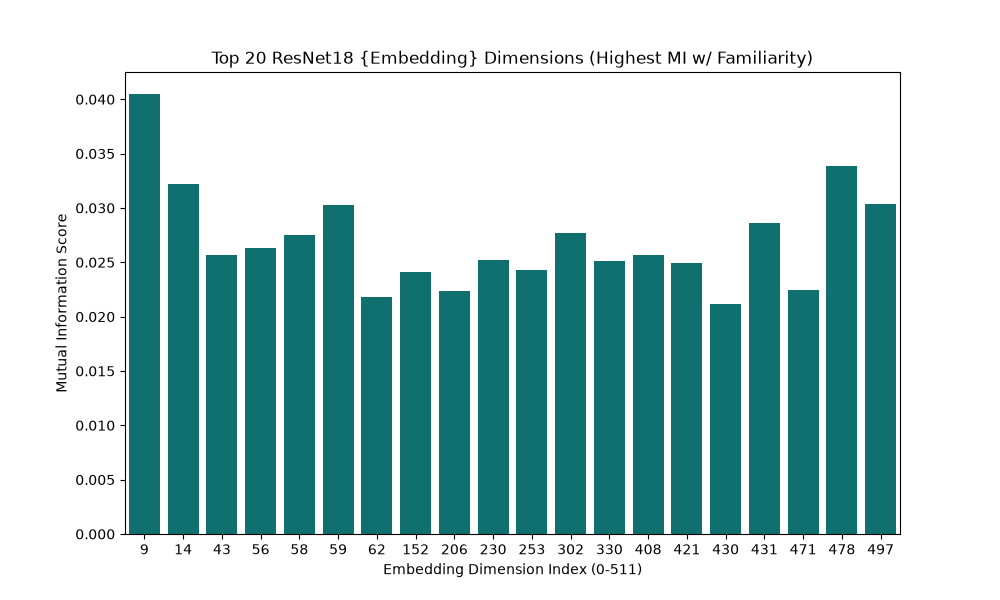
\includegraphics[width=\linewidth]{5Epoch_plantNet_Trained_ResNet18_Embedding_MIScore.png}
\caption{ResNet-18 (top 20 of 512 dimensions)}
\label{fig:mi_resnet}
\end{subfigure}
\hfill
\begin{subfigure}{0.49\textwidth}
\centering
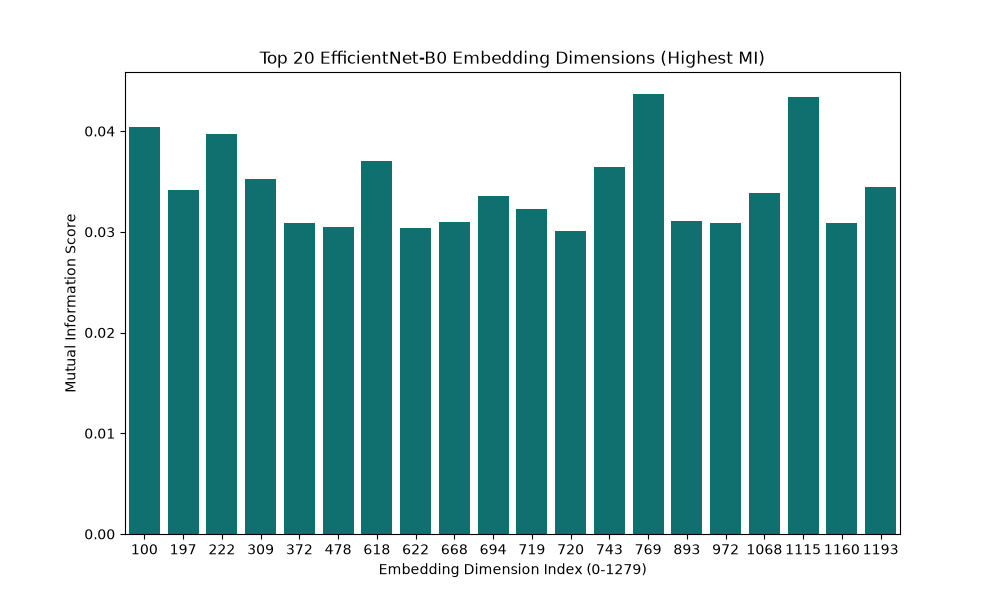
\includegraphics[width=\linewidth]{10Epoch_plantNet_Trained_EfficientNetB0_Embedding_MIScore.png}
\caption{EfficientNet-B0 (top 20 of 1,280 dimensions)}
\label{fig:mi_effnet}
\end{subfigure}
\caption{Mutual information between individual embedding dimensions and the known/unknown familiarity label, after fine-tuning. Note the small vertical scale: the most informative single dimension carries well under 0.05 nats, against a maximum of $\ln 2 \approx 0.693$.}
\label{fig:mi}
\end{figure}

The results are strikingly similar across the two architectures, and the key observation is how \emph{small} the scores are. Even the single most informative dimension reaches a mutual information of only about 0.040 for ResNet-18 (dimension 9) and 0.044 for EfficientNet-B0 (dimension 769), against a theoretical maximum of $\ln 2 \approx 0.693$ for a balanced binary label. The top twenty dimensions are also tightly clustered in value, with no dominant feature standing out from the rest.

Two conclusions follow. First, no individual neuron functions as a novelty detector, so any effective open-set method must aggregate evidence across the full embedding vector rather than monitor a small set of features. Second, the near-uniformity of the top scores indicates that the familiarity signal is distributed diffusely across hundreds of weakly informative dimensions. This is precisely the regime in which whitened, full-covariance distance measures should outperform methods that treat dimensions independently, and the open-set results in Section~\ref{sec:osr_results} bear this out.

\subsubsection{PCA Projection}

We next projected the high-dimensional embeddings onto their first two principal components, colouring each point by familiarity.

\begin{figure}[htbp]
\centering
\begin{subfigure}{0.49\textwidth}
\centering
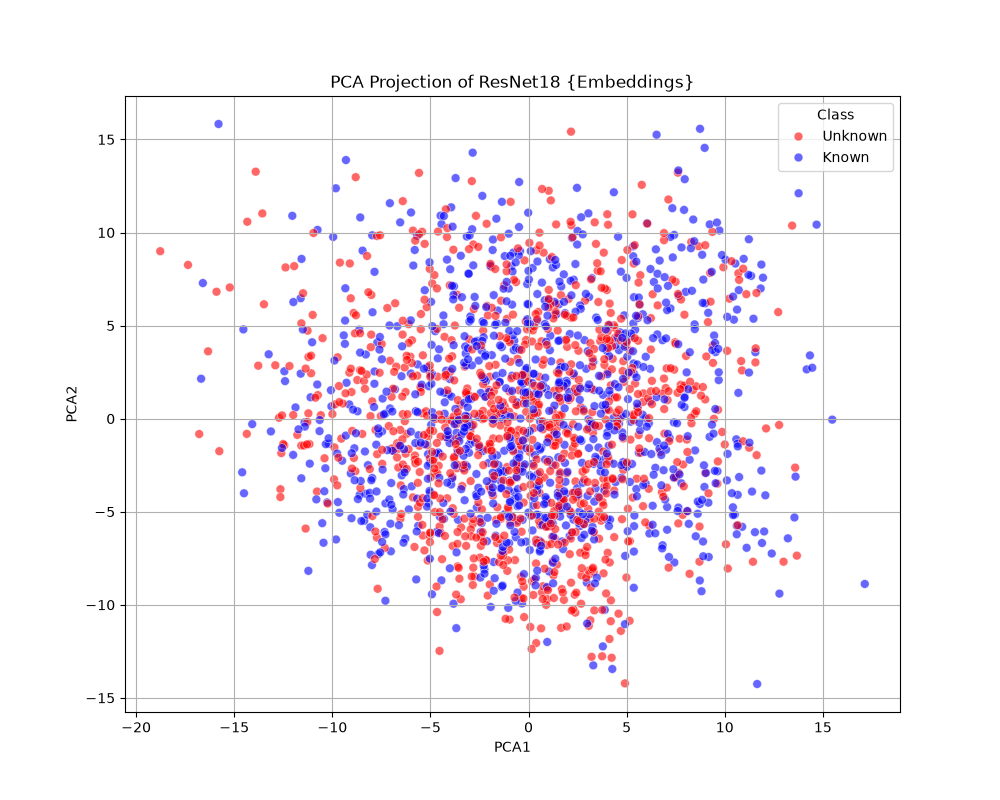
\includegraphics[width=\linewidth]{5Epoch_plantNet_Trained_ResNet18_Embedding_PCA_Projection.png}
\caption{ResNet-18}
\label{fig:pca_resnet}
\end{subfigure}
\hfill
\begin{subfigure}{0.49\textwidth}
\centering
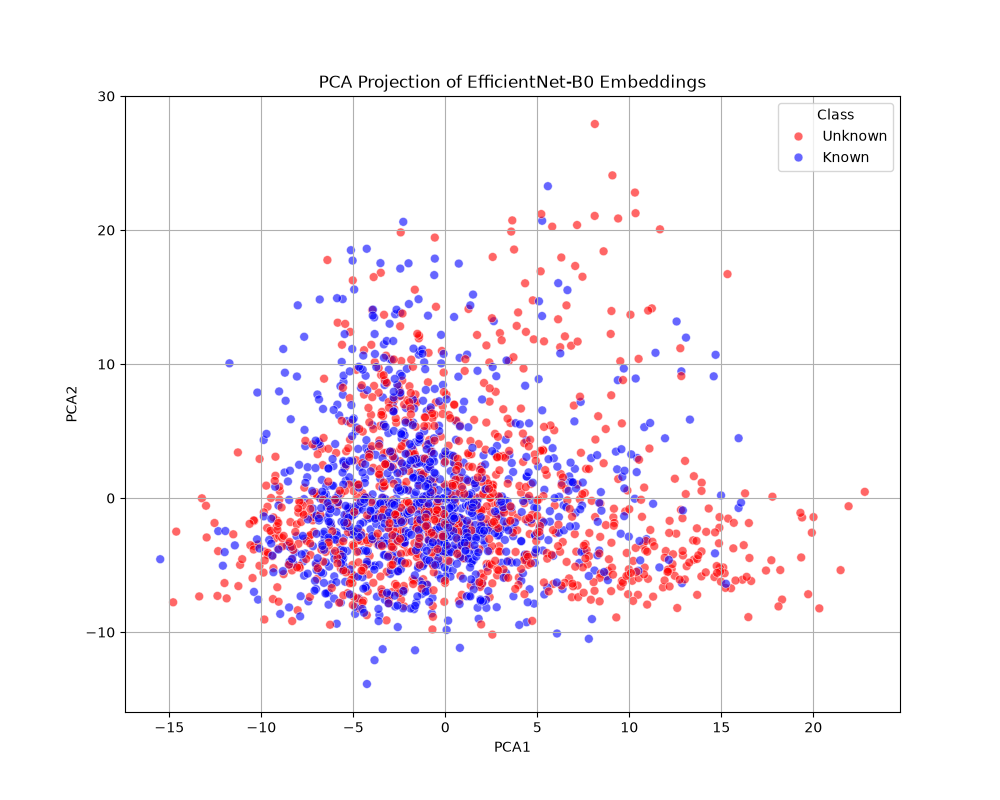
\includegraphics[width=\linewidth]{10Epoch_plantNet_Trained_EfficientNetB0_Embedding_PCA_Projection.png}
\caption{EfficientNet-B0}
\label{fig:pca_effnet}
\end{subfigure}
\caption{PCA projection of the learned embeddings onto the first two principal components, coloured by known versus unknown species. The two groups overlap almost completely in both cases.}
\label{fig:pca}
\end{figure}

Neither projection shows two separated groups. Known and unknown species occupy the same region of the plane and overlap almost completely, confirming that novelty is not captured by the directions of greatest variance. This is an expected but important negative result: the leading principal components of a fine-tuned network encode the dominant sources of visual variation in plant photographs -- illumination, background, viewpoint, and organ type -- and these vary just as much within the known species as between known and unknown ones.

The EfficientNet-B0 projection (Figure~\ref{fig:pca_effnet}) does show a subtle asymmetry that the ResNet-18 projection lacks: the known species form a denser core near the origin, while unknown species are somewhat more likely to appear in the diffuse right-hand tail along the first component. This is consistent with EfficientNet-B0's stronger open-set performance, but the effect is far too weak to support a decision rule in two dimensions. Together, Figures~\ref{fig:mi} and~\ref{fig:pca} establish that open-set recognition here requires methods that operate on the full high-dimensional geometry, which motivates the scorers evaluated next.

\subsubsection{Activation Fingerprints}

Finally, activation fingerprint visualizations were generated for the first sixteen evaluation images to compare the internal representations learned by the two architectures.

\begin{figure}[htbp]
\centering
\begin{subfigure}{0.49\textwidth}
\centering
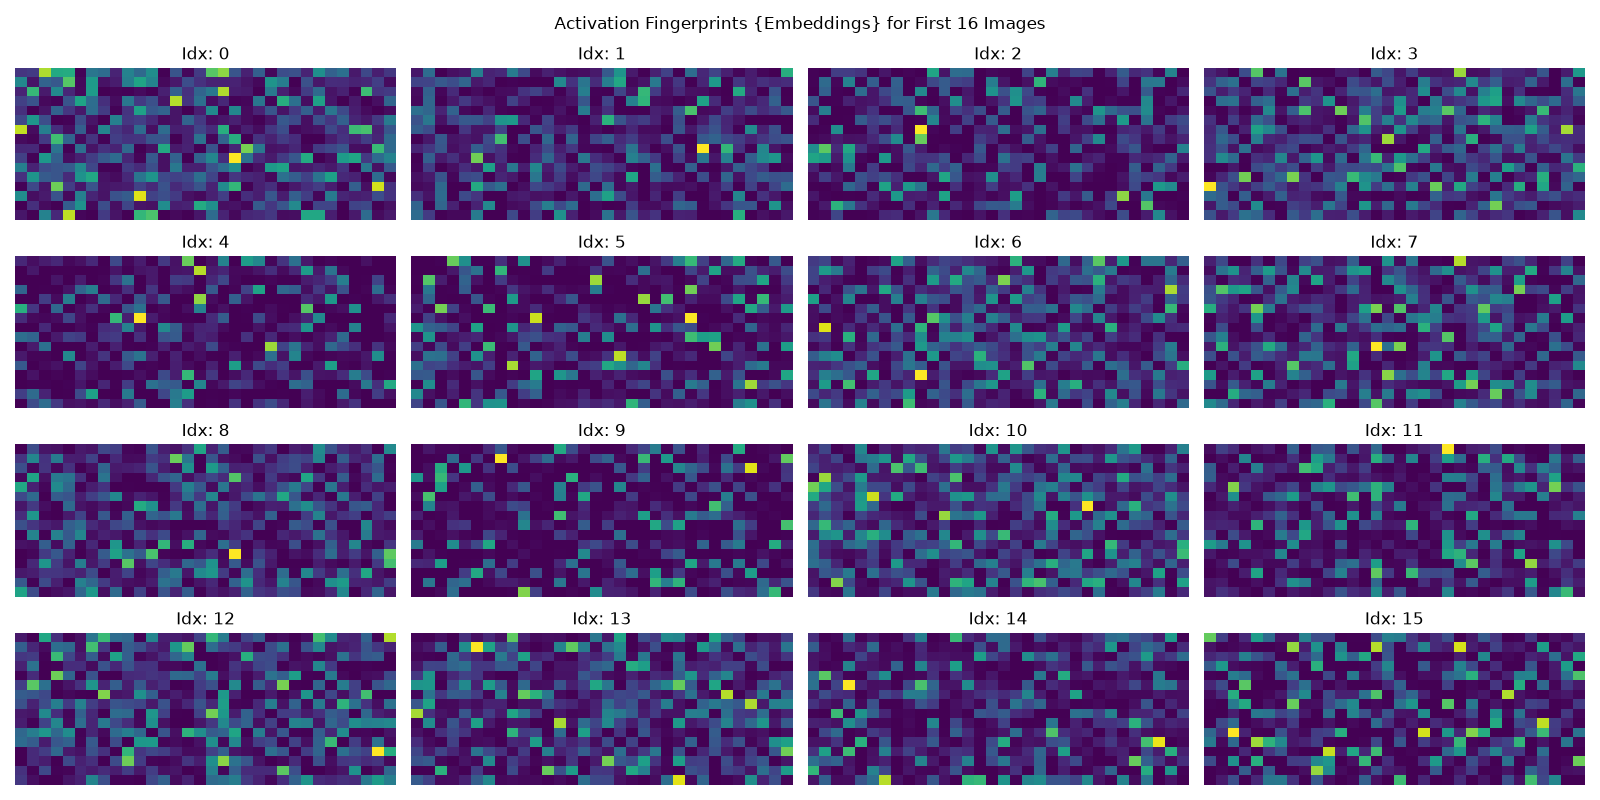
\includegraphics[width=\linewidth]{5Epoch_plantNet_Trained_ResNet18_Embedding_Activation_FingerPrints_First_16Images.png}
\caption{ResNet-18}
\label{fig:fp_resnet}
\end{subfigure}
\hfill
\begin{subfigure}{0.49\textwidth}
\centering
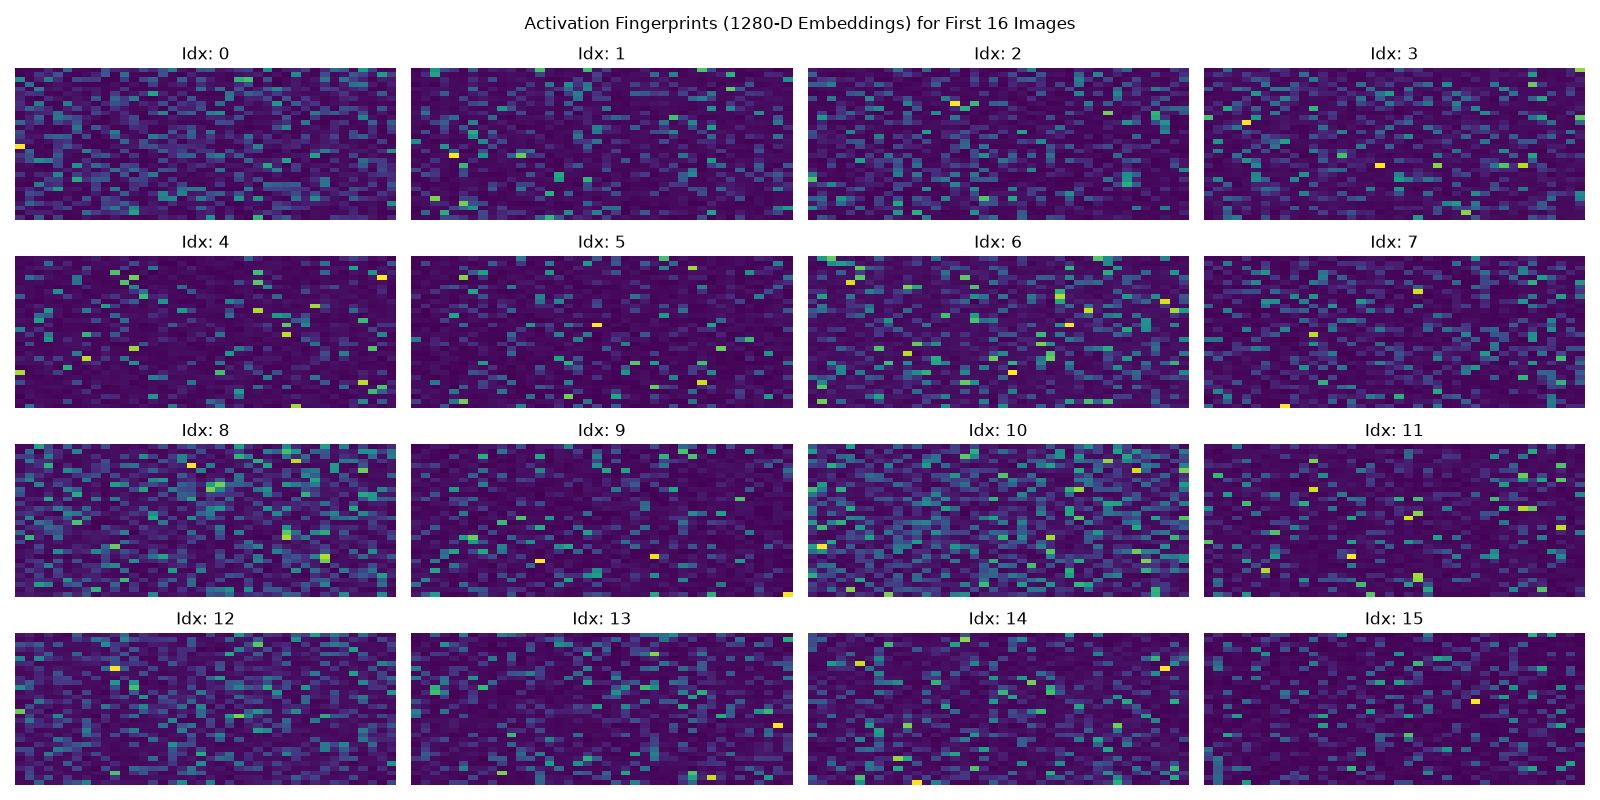
\includegraphics[width=\linewidth]{10Epoch_plantNet_Trained_EfficientNetB0_Embedding_Activation_FingerPrints_First_16Images.png}
\caption{EfficientNet-B0}
\label{fig:fp_effnet}
\end{subfigure}
\caption{Activation fingerprints of the first 16 evaluation images after fine-tuning. Both networks produce sparse, image-specific patterns with no visually obvious distinction between known and unknown species.}
\label{fig:fp}
\end{figure}

Both networks produce sparse, highly non-negative activation patterns, a consequence of the ReLU non-linearity preceding the pooled embedding layer. The fingerprints differ visibly from image to image, confirming that the representations are image-specific rather than collapsed, but the patterns for known and unknown species are not qualitatively distinguishable by eye. This reinforces the conclusion drawn from the mutual information analysis: the distinction between familiar and unfamiliar species is a subtle, distributed property of the embedding rather than a visually obvious one.

\subsection{Open-Set Recognition Performance}
\label{sec:osr_results}

We now turn to the central question of the project: how reliably can each method identify images of the 45 species that were withheld from training? All seven scorers were applied to the same balanced evaluation set of 2,000 known-species and 2,000 unknown-species images, for both backbones. Table~\ref{tab:osr_results} reports the results, and Figure~\ref{fig:roc} shows the corresponding ROC curves.

\begin{table}[H]
\centering
\caption{Open-set detection performance. The positive class is ``unfamiliar''; ROC AUC of 0.5 is chance. FPR@95 is the false positive rate at the threshold achieving 95\% true positive rate (lower is better). Best value in each column is in bold.}
\label{tab:osr_results}

\begin{tabular}{lcccc}
\toprule
& \multicolumn{2}{c}{ResNet-18 (512-d)} & \multicolumn{2}{c}{EfficientNet-B0 (1280-d)} \\
\cmidrule(lr){2-3}\cmidrule(lr){4-5}
Scorer & ROC AUC & FPR@95 & ROC AUC & FPR@95 \\
\midrule
MSP (baseline)        & 0.625 & 0.880 & 0.620 & 0.848 \\
Energy                & 0.708 & 0.808 & 0.730 & 0.862 \\
Mahalanobis           & 0.621 & 0.869 & 0.725 & 0.747 \\
Mahalanobis ($L_2$)   & 0.740 & 0.765 & 0.766 & 0.747 \\
$k$NN, $k{=}5$ ($L_2$) & \textbf{0.755} & \textbf{0.747} & \textbf{0.790} & \textbf{0.692} \\
One-Class SVM         & 0.364 & 0.986 & 0.489 & 0.954 \\
Isolation Forest      & 0.394 & 0.980 & 0.564 & 0.908 \\
\bottomrule
\end{tabular}
\end{table}

\begin{figure}[htbp]
\centering
\begin{subfigure}{0.49\textwidth}
\centering
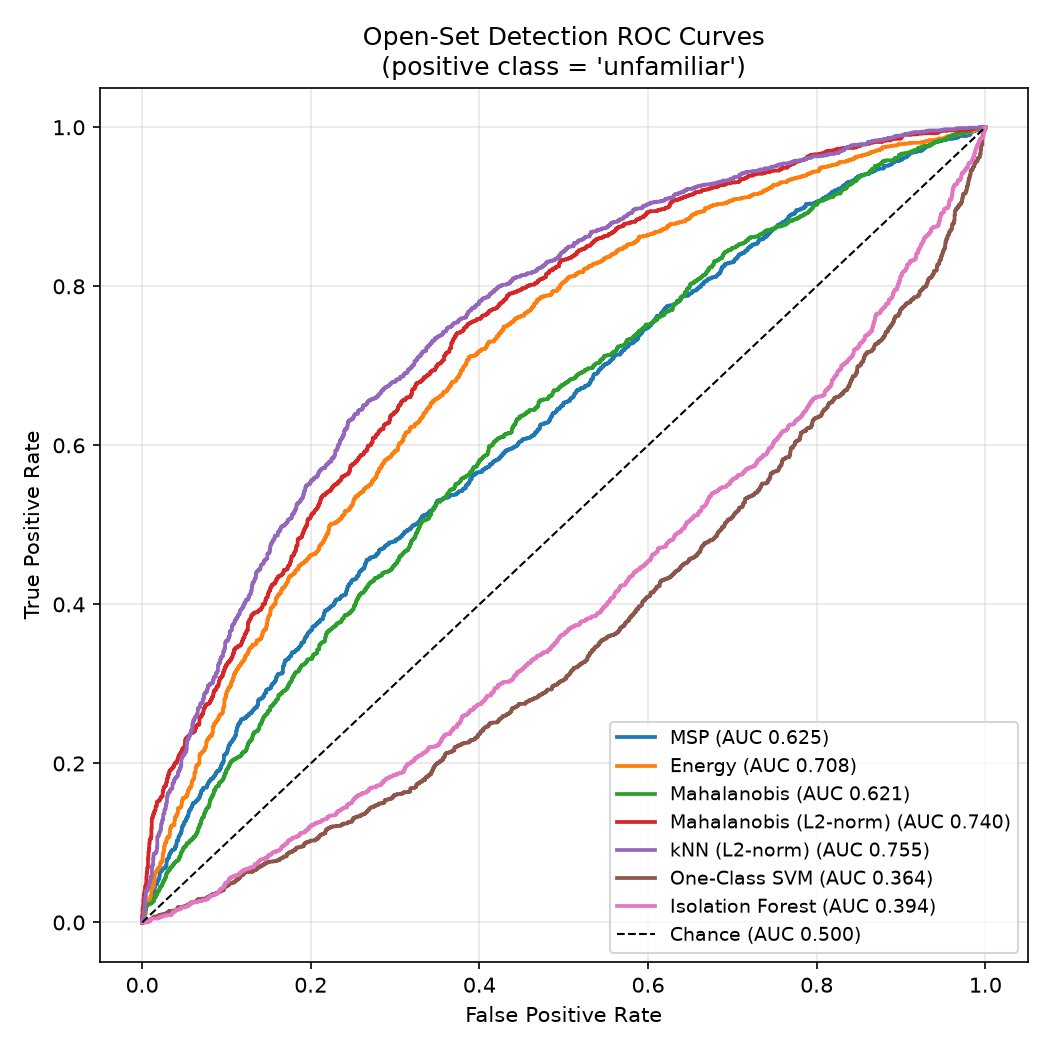
\includegraphics[width=\linewidth]{roc_curves.png}
\caption{ResNet-18}
\label{fig:roc_resnet}
\end{subfigure}
\hfill
\begin{subfigure}{0.49\textwidth}
\centering
\includegraphics[width=\linewidth]{roc_curves_effnet.png}
\caption{EfficientNet-B0}
\label{fig:roc_effnet}
\end{subfigure}
\caption{Open-set detection ROC curves for all seven scorers, with ``unfamiliar'' as the positive class. The dashed diagonal is chance. Note that the One-Class SVM and Isolation Forest curves fall \emph{below} the diagonal for ResNet-18.}
\label{fig:roc}
\end{figure}

Four findings stand out.

\textbf{Embedding geometry beats classifier confidence.} The MSP baseline is the weakest of the usable methods on both backbones, reaching an ROC AUC of only 0.625 for ResNet-18 and 0.620 for EfficientNet-B0. The best method, $k$-nearest neighbour distance on $L_2$-normalized embeddings, reaches 0.755 and 0.790 respectively, improving on the baseline by 13 and 17 AUC points. The energy score, which uses the full logit vector rather than only its maximum, recovers a substantial part of this gap (0.708 and 0.730) at no extra cost, confirming that much of MSP's weakness comes from discarding information when the softmax is normalized. Notably, MSP is the one scorer that does \emph{not} improve with the stronger backbone, which suggests that softmax confidence saturates in a way that is largely independent of representation quality.

\textbf{$L_2$ normalization is the single most valuable preprocessing step.} Normalizing embeddings to unit length before computing Mahalanobis distance raises the AUC from 0.621 to 0.740 for ResNet-18 and from 0.725 to 0.766 for EfficientNet-B0. The gain of nearly 12 points for ResNet-18 exceeds the benefit of switching to the larger architecture. Discarding feature magnitude and comparing embeddings only by direction is therefore a substantially better representation of novelty, a point developed in Section~\ref{sec:discussion}.

\textbf{The stronger backbone is better for open-set detection, not just classification.} EfficientNet-B0 outperforms ResNet-18 on six of the seven scorers, and the ranking of methods is nearly identical across the two. The 5.9-point advantage in closed-set validation accuracy thus translates into a genuinely more novelty-aware embedding space rather than merely a better decision boundary among the known classes. The consistency of the method ranking across two architectures also indicates that these conclusions are properties of the scorers rather than artifacts of one network.

\textbf{Global one-class methods fail outright.} One-Class SVM and Isolation Forest perform at or below chance on both backbones. On ResNet-18 embeddings they achieve AUCs of 0.364 and 0.394, meaning that a randomly chosen unknown-species image is systematically ranked as \emph{more} typical of the training distribution than a randomly chosen known-species image. This is not a sign convention error -- both scorers are oriented so that higher values mean more anomalous -- but a real and reproducible inversion. Section~\ref{sec:discussion} isolates its cause with two controlled ablations, and the answer turns out to explain why the successful scorers succeed.

Finally, the absolute difficulty of the task deserves emphasis. Even the best configuration requires flagging 69\% of known-species images in order to catch 95\% of the unknown ones, and the corresponding F1 at that operating point is 0.72. Fine-grained novelty detection among visually similar plant species is therefore far harder than the coarse out-of-distribution benchmarks on which these methods are usually reported.

\subsubsection{Statistical Reliability}

The AUC values above are point estimates from a single held-out species partition, so we quantified their uncertainty with a species-level bootstrap. Table~\ref{tab:bootstrap} reports the mean and a 95\% percentile interval over 2,000 resamples in which entire species, rather than individual images, were drawn with replacement.

\begin{table}[H]
\centering
\caption{Species-level bootstrap 95\% confidence intervals for ROC AUC, over 2,000 resamples of whole species. Identical resamples were used for every scorer so that comparisons are paired.}
\label{tab:bootstrap}

\begin{tabular}{lcc}
\toprule
& ResNet-18 & EfficientNet-B0 \\
Scorer & Mean AUC [95\% CI] & Mean AUC [95\% CI] \\
\midrule
MSP (baseline)         & 0.625 [0.571, 0.680] & 0.620 [0.554, 0.686] \\
Energy                 & 0.708 [0.658, 0.759] & 0.730 [0.670, 0.793] \\
Mahalanobis            & 0.623 [0.535, 0.694] & 0.727 [0.645, 0.788] \\
Mahalanobis ($L_2$)    & 0.742 [0.675, 0.797] & 0.768 [0.690, 0.836] \\
$k$NN, $k{=}5$ ($L_2$) & 0.757 [0.697, 0.812] & 0.792 [0.728, 0.855] \\
One-Class SVM          & 0.364 [0.313, 0.421] & 0.489 [0.423, 0.557] \\
Isolation Forest       & 0.396 [0.328, 0.459] & 0.564 [0.501, 0.626] \\
\bottomrule
\end{tabular}
\end{table}

The intervals are wide, spanning roughly 0.11 to 0.15 AUC, which confirms that a single point estimate on 45 held-out species should not be over-interpreted. They nevertheless separate the main conclusions cleanly. For EfficientNet-B0 the interval for the $k$-nearest neighbour scorer, $[0.728, 0.855]$, lies entirely above that of the MSP baseline, $[0.554, 0.686]$, so the advantage of embedding-based detection over classifier confidence is not an artifact of the particular species drawn. Likewise, the One-Class SVM interval on ResNet-18 embeddings, $[0.313, 0.421]$, lies entirely below 0.5: the below-chance inversion is statistically robust rather than sampling noise, which is what motivated the diagnostic analysis in Section~\ref{sec:discussion}. By contrast, the same scorer on EfficientNet-B0 spans 0.5 at $[0.423, 0.557]$ and is therefore indistinguishable from random guessing, and the Isolation Forest interval of $[0.501, 0.626]$ only barely excludes it. Neither one-class method can be considered useful on either backbone.

\subsection{Effect of Taxonomic Similarity}
\label{sec:taxonomy}

Our proposal predicted that detection would be hardest when an unfamiliar species is taxonomically close to a known one, since such plants are visually similar and should lie near the known-class clusters in feature space. We tested this directly by splitting the 45 held-out species according to genus. Of these, 32 species (1,433 test images) belong to a genus that also appears among the 181 known species, while 13 species (567 images) come from a genus the network never saw. A separate AUC was computed for each group against the same known-species images, so the two values are directly comparable.

\begin{table}[H]
\centering
\caption{ROC AUC by taxonomic distance. Same-genus unknowns belong to a genus represented in the training set; novel-genus unknowns do not. $\Delta$ is the novel-genus advantage; positive values mean same-genus species are harder to detect.}
\label{tab:taxonomy}

\begin{tabular}{lccc@{\hspace{1.2em}}ccc}
\toprule
& \multicolumn{3}{c}{ResNet-18} & \multicolumn{3}{c}{EfficientNet-B0} \\
\cmidrule(lr){2-4}\cmidrule(lr){5-7}
Scorer & Same & Novel & $\Delta$ & Same & Novel & $\Delta$ \\
\midrule
MSP (baseline)         & 0.601 & 0.687 & $+0.086$ & 0.587 & 0.706 & $+0.119$ \\
Energy                 & 0.679 & 0.781 & $+0.102$ & 0.694 & 0.821 & $+0.128$ \\
Mahalanobis            & 0.601 & 0.673 & $+0.072$ & 0.701 & 0.785 & $+0.084$ \\
Mahalanobis ($L_2$)    & 0.715 & 0.803 & $+0.088$ & 0.725 & 0.868 & $+0.143$ \\
$k$NN, $k{=}5$ ($L_2$) & 0.718 & 0.850 & $+0.133$ & 0.748 & 0.897 & $+0.149$ \\
One-Class SVM          & 0.366 & 0.358 & $-0.008$ & 0.507 & 0.445 & $-0.062$ \\
Isolation Forest       & 0.382 & 0.425 & $+0.043$ & 0.562 & 0.570 & $+0.009$ \\
\bottomrule
\end{tabular}
\end{table}

The hypothesis is confirmed, and the effect is large. Every scorer that performs better than chance detects novel-genus species more reliably than same-genus ones, on both backbones without exception. For the best configuration, EfficientNet-B0 with $k$-nearest neighbour scoring, AUC falls from 0.897 on novel-genus species to 0.748 on same-genus species, a drop of 0.149. Detecting a plant from an entirely unseen genus is therefore close to a solved problem at this scale, while distinguishing a new species from its own known relatives remains substantially harder.

Two further details are worth noting. The gap is largest precisely for the strongest scorers -- 0.149 and 0.143 for the two best EfficientNet-B0 configurations, against 0.084 for unnormalized Mahalanobis distance -- which indicates that the better methods gain most of their advantage on the taxonomically distant cases and that all methods converge toward similar difficulty on close relatives. This also means the aggregate AUC figures in Table~\ref{tab:osr_results} depend on the taxonomic composition of the held-out set: because 71\% of our unknown species share a genus with a known species, those aggregate numbers are dominated by the hard regime, and a benchmark weighted toward distant novelties would report considerably better performance.

The two one-class methods again behave differently from everything else, showing no meaningful taxonomic effect and in fact a slightly \emph{negative} gap. A method that genuinely measured novelty could not be indifferent to taxonomic distance in this way, which independently corroborates the conclusion of Section~\ref{sec:discussion} that these scorers respond to something other than novelty.

\subsection{Sensitivity to Test-Time Openness}
\label{sec:openness}

Finally, we varied the number of distinct unknown species appearing in the evaluation set from 5 to 45, holding the known-species images fixed and averaging over 200 random subsamples at each level. Figure~\ref{fig:openness} shows the result for the best scorer on both backbones.

\begin{figure}[H]
\centering
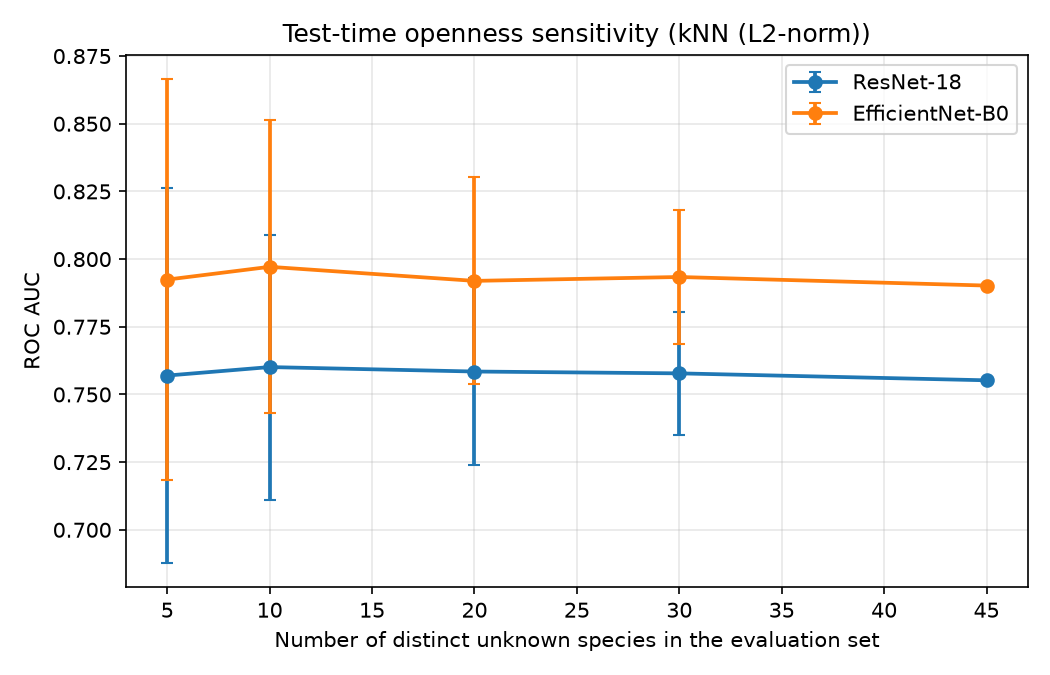
\includegraphics[width=.72\linewidth]{openness_sweep.png}
\caption{ROC AUC as a function of the number of distinct unknown species present in the evaluation set, for $k$-nearest neighbour scoring. Error bars show one standard deviation across 200 random subsamples of the held-out species.}
\label{fig:openness}
\end{figure}

Mean AUC is essentially flat across the whole range, moving only between 0.755 and 0.760 for ResNet-18 and between 0.790 and 0.797 for EfficientNet-B0. The detector's accuracy therefore does not degrade as the evaluation stream becomes more diverse, and the gap between the two backbones persists at every level. What changes sharply is the variability: the standard deviation across subsamples falls from 0.069 with five unknown species to 0.025 with thirty. Evaluations built on only a handful of held-out species are consequently unreliable, which reinforces the value of the confidence intervals in Table~\ref{tab:bootstrap} and explains why the taxonomic composition analysed in Section~\ref{sec:taxonomy} matters so much when the unknown pool is small.

\subsection{Discussion}
\label{sec:discussion}

The most informative result is the failure of the two global one-class methods, because diagnosing it explains why the successful methods succeed. We approached it as a hypothesis-testing exercise, and the first hypothesis we tried turned out to be wrong, which is worth reporting because it changes the conclusion.

\subsubsection{First Hypothesis: Embedding Magnitude}

One-Class SVM and Isolation Forest differ from the Mahalanobis and $k$-nearest neighbour scorers in two respects. They operate on standardized rather than length-normalized embeddings, so their notion of ``typical'' is influenced by the magnitude of the activation vector; and they ignore the class labels, modelling all 181 known species as one undifferentiated cloud.

The magnitude explanation initially looked compelling. For ResNet-18, known-species evaluation images have a mean $L_2$ norm of 32.85, closely matching the known training images at 32.87, while unknown-species images average only 31.26. Using embedding norm alone as a novelty score, with smaller norms taken to indicate unfamiliarity, yields an AUC of 0.594 -- well above chance. Unknown-species images do elicit measurably weaker activations, which places them nearer the centre of the standardized feature cloud, precisely where a density estimator judges a point to be most normal.

This account makes a falsifiable prediction: removing magnitude by projecting embeddings onto the unit sphere before fitting should rescue both methods. Table~\ref{tab:ablation} reports that test.

\begin{table}[H]
\centering
\caption{Normalization ablation. Each detector is fitted twice on identical data, once on standardized embeddings and once on $L_2$-normalized embeddings, so the only difference is whether magnitude information survives. Removing magnitude does not rescue either method.}
\label{tab:ablation}

\begin{tabular}{llccc}
\toprule
Backbone & Method & Standardized & $L_2$-normalized & Change \\
\midrule
\multirow{2}{*}{ResNet-18}
 & One-Class SVM    & 0.364 & 0.358 & $-0.006$ \\
 & Isolation Forest & 0.394 & 0.434 & $+0.040$ \\
\midrule
\multirow{2}{*}{EfficientNet-B0}
 & One-Class SVM    & 0.489 & 0.404 & $-0.086$ \\
 & Isolation Forest & 0.564 & 0.577 & $+0.013$ \\
\bottomrule
\end{tabular}
\end{table}

The prediction fails. Normalization leaves the One-Class SVM essentially unchanged on ResNet-18 ($-0.006$) and makes it distinctly \emph{worse} on EfficientNet-B0 ($-0.086$), while Isolation Forest improves only marginally and remains below chance on ResNet-18. Magnitude is therefore correlated with novelty in these embeddings, but it is not what causes the one-class methods to fail. The first hypothesis is refuted.

\subsubsection{Second Hypothesis: Loss of Class-Conditioning}

The remaining structural difference is class-conditioning. To test it in isolation we compared two scorers that are identical in geometry, metric, and preprocessing -- Euclidean distance on $L_2$-normalized embeddings -- and differ only in how many reference points they use: a single global centroid, or the nearest of the 181 class centroids. Table~\ref{tab:centroid} gives the result.

\begin{table}[H]
\centering
\caption{Isolating class-conditioning. Both scorers use Euclidean distance on $L_2$-normalized embeddings; the only difference is the number of reference points. Class-conditioning alone accounts for roughly 0.40 AUC.}
\label{tab:centroid}

\begin{tabular}{lcc}
\toprule
Reference points & ResNet-18 & EfficientNet-B0 \\
\midrule
Single global centroid          & 0.347 & 0.394 \\
Nearest of 181 class centroids  & 0.749 & 0.783 \\
\midrule
Difference                      & $+0.401$ & $+0.389$ \\
\bottomrule
\end{tabular}
\end{table}

The effect is unambiguous and very large. Holding everything else fixed, replacing 181 class centroids with a single global one moves AUC by roughly 0.40, turning a useful detector into a below-chance one. The global-centroid figures also closely track the one-class methods they are meant to model: 0.347 against 0.364 for the One-Class SVM on ResNet-18, and 0.394 against exactly 0.394 for Isolation Forest. Whatever the kernel or the tree ensemble is nominally doing, its practical behaviour is well approximated by distance from the global mean.

\subsubsection{A Unified Account}

Together these two experiments support a single coherent explanation. Fine-tuning reshapes the embedding space so that confidently recognized inputs are driven \emph{away} from the global mean, along directions specific to their class, while inputs the network cannot commit to produce weak, non-committal representations that remain near the average of everything. Distance from the global centre therefore measures the network's confidence, not the input's novelty, and it does so with the wrong sign: unfamiliar species look \emph{more} central, not less. This is why every global measure we tried lands in the same below-chance band for ResNet-18 -- One-Class SVM at 0.364, Isolation Forest at 0.394, global-centroid distance at 0.347 -- and why the embedding-norm correlation we observed first was a symptom of this geometry rather than its cause.

Novelty becomes visible only when an observation is compared against the known classes \emph{individually}. An unfamiliar species does not sit outside the region occupied by the training data; it sits in the gaps \emph{between} class clusters, which are interior to the global support and therefore invisible to any method modelling that support as one region. Class-conditional scorers measure distance to the nearest cluster and detect exactly this, which is why they cluster in the 0.74--0.79 band. The further gain from $k$-nearest neighbours over class centroids follows the same logic taken one step further: a species photographed as flower, leaf, fruit, and whole plant forms several distinct clusters that a single mean per class cannot represent, and local distances can.

This also reframes the role of $L_2$ normalization. It is genuinely valuable for the class-conditional scorers, worth up to 12 AUC points for Mahalanobis distance, because it removes a nuisance direction that would otherwise dilute the class-relative signal. But Table~\ref{tab:ablation} shows it cannot repair a scorer whose fundamental structure is wrong. Normalization improves a method that is asking the right question; it does not change the question being asked.

\subsubsection{Implications}

The taxonomic analysis in Section~\ref{sec:taxonomy} fits this account and sharpens it. If the successful scorers work by measuring distance to the nearest known class in angular geometry, then their difficulty should scale with how close the nearest known class actually is -- and it does, with AUC dropping by 0.149 when the unfamiliar species belongs to a genus the model already knows. Congeneric species share leaf shape, inflorescence structure, and growth habit, so their embeddings fall near or inside the cluster of their known relative, and no purely geometric criterion can separate them cleanly. This also reframes the aggregate results: the headline AUC of 0.790 is not a single difficulty level but an average over an easy regime, where detection approaches 0.90, and a hard regime, where it is closer to 0.75.

These findings carry a practical implication for biodiversity screening. A deployed system should compare a new observation against the known species \emph{individually}, using normalized embeddings and local distances, rather than asking whether the observation resembles the training set as a whole. At the same time, an FPR of 0.69 at 95\% recall means such a system cannot function as an automatic filter. Its realistic use is as a ranking tool: sorting incoming observations by unfamiliarity score so that experts examine the most suspicious specimens first, which the AUC of 0.79 indicates would be considerably more efficient than reviewing observations in arbitrary order.

Encouragingly for that use case, the openness sweep in Section~\ref{sec:openness} shows that performance is stable regardless of how many distinct novel species arrive, so the ranking would not degrade as a deployment encounters more varied flora. The taxonomic result, however, implies a specific and predictable blind spot: such a system would be least sensitive to precisely the novelties that are easiest to mistake for known plants, and a genuinely novel congener could pass through with a low unfamiliarity score. Where the goal is to catch new members of well-surveyed genera, geometric novelty detection on its own is unlikely to suffice, and the taxonomic or geographic metadata discussed below becomes correspondingly more valuable.

\section{Limitations}
\label{sec:limitations}

Several limitations should be considered when interpreting the results of this study. First, the evaluation was conducted using a curated subset of the Pl@ntNet-300K dataset, meaning that the learned models were exposed only to relatively well-represented species. Although this improves training stability, it does not fully reflect the long-tailed distribution encountered in real-world biodiversity monitoring. The unknown species were drawn from the same well-represented pool, so they are comparatively easy cases; genuinely rare species would likely be harder still.

Second, the two architectures were fine-tuned for different numbers of epochs, five for ResNet-18 and ten for EfficientNet-B0. The comparison between them therefore confounds architecture with training budget, and the consistent advantage of EfficientNet-B0 cannot be attributed to architecture alone. Because the ranking of open-set methods is essentially identical across both backbones, this confound does not affect the study's principal conclusions, which concern the relative merits of the scorers rather than of the networks.

Third, and most importantly, all results rest on a \emph{single} species-level partition into known and unknown sets. Our proposal planned to repeat this partition several times and report variability across runs, but each new partition changes which species the networks were trained on and therefore requires retraining both backbones from scratch. At approximately 385 and 6,780 minutes per model, even a handful of partitions was beyond the computational budget available. The species-level bootstrap in Table~\ref{tab:bootstrap} and the openness sweep in Section~\ref{sec:openness} are deliberate substitutes and should be read as such: the bootstrap captures uncertainty from \emph{which held-out species were drawn} into the evaluation set, and the sweep captures sensitivity to \emph{how many} novel species appear at test time, but neither captures the variability introduced by training the network on a different set of known species. The reported confidence intervals are therefore lower bounds on the true uncertainty, and the intervals of 0.11 to 0.15 already caution against fine-grained comparisons between closely ranked scorers.

Fourth, the open-set scorers were compared using threshold-free metrics and a single fixed operating point, without tuning their hyperparameters. The One-Class SVM used a fixed $\nu = 0.1$ with an RBF kernel and the $k$-nearest neighbour scorer a fixed $k = 5$, so a hyperparameter search could change their standing. We did test one such variation directly -- fitting the one-class methods on $L_2$-normalized instead of standardized embeddings -- and Table~\ref{tab:ablation} shows it does not help, but we cannot rule out that a different kernel bandwidth or a per-class one-class formulation would perform considerably better. The analysis in Section~\ref{sec:discussion} suggests the latter specifically: a one-class model fitted separately to each known species would retain the class-conditioning that we identify as the decisive factor, and would be the natural next experiment.

Fifth, all unknown species originated from the same dataset as the known species. While this provides a controlled evaluation protocol, future work should investigate generalization to completely independent datasets collected under different environmental conditions. Section~\ref{sec:taxonomy} also shows that the aggregate figures depend on the taxonomic composition of the held-out set, so results from studies using differently composed unknown sets are not directly comparable to ours.

Finally, the open-set recognition methods operate exclusively on visual information. Incorporating additional metadata, such as geographic location, seasonality, or taxonomic relationships, could further improve the detection of unfamiliar species.

\section{Conclusion}


This project investigated open-set recognition for plant species identification using deep feature representations learned from convolutional neural networks. A curated subset of the Pl@ntNet-300K dataset was used to train image classification models while intentionally excluding a subset of species to simulate unfamiliar observations during evaluation.

Transfer learning with ResNet-18 and EfficientNet-B0 produced discriminative feature embeddings suitable for both classification and open-set recognition, reaching 72.3\% and 78.2\% validation accuracy across 181 known species. Representation analysis showed that familiarity is not encoded by any individual embedding dimension, nor along the directions of greatest variance, establishing that open-set detection here requires methods operating on the full high-dimensional geometry.

Comparing seven detection methods produced four concrete conclusions. Distance-based scorers operating on $L_2$-normalized embeddings clearly outperform classifier confidence, with $k$-nearest neighbour distance reaching an ROC AUC of 0.790 against 0.620 for the Maximum Softmax Probability baseline, a separation confirmed by non-overlapping bootstrap confidence intervals. Length normalization is the single most valuable preprocessing step, worth up to 12 AUC points on its own. Most instructively, global one-class methods performed at or below chance, and two controlled ablations identified why. The intuitive explanation, embedding magnitude, proved wrong: projecting the embeddings onto the unit sphere failed to rescue either method. The actual cause is the loss of class-conditioning. Substituting a single global centroid for the 181 class centroids, with metric and preprocessing held fixed, shifts AUC by roughly 0.40 and reproduces the failure almost exactly. Unfamiliar species sit in the gaps between known class clusters rather than outside the training distribution as a whole, so only methods that compare an observation against each known species individually can detect them.

Finally, the difficulty of the task depends strongly on taxonomy, confirming the hypothesis set out in our proposal. Detection AUC falls from 0.897 for species belonging to an entirely unseen genus to 0.748 for species whose genus the model already knows. Recognizing a plant from an unfamiliar branch of the tree of life is comparatively easy; recognizing a new species among its own known relatives is the real challenge, and it is the case that matters most for surveying well-studied floras.

Overall, this work demonstrates that combining deep feature extraction with open-set recognition offers a practical framework for biodiversity screening, provided the detector respects the geometry of the embedding space. Given a false positive rate of 0.69 at 95\% recall, the realistic application is not an automatic filter but a triage tool that ranks incoming observations by unfamiliarity so that experts examine the most unusual specimens first. Future work will investigate metric-learning objectives that shape the embedding space explicitly for novelty detection, hyperparameter tuning and normalization for the one-class methods, and validation against species drawn from entirely independent collections.

\bibliographystyle{plain}
\bibliography{references}



\end{document}